
\subsection*{1.}

\begin{center}
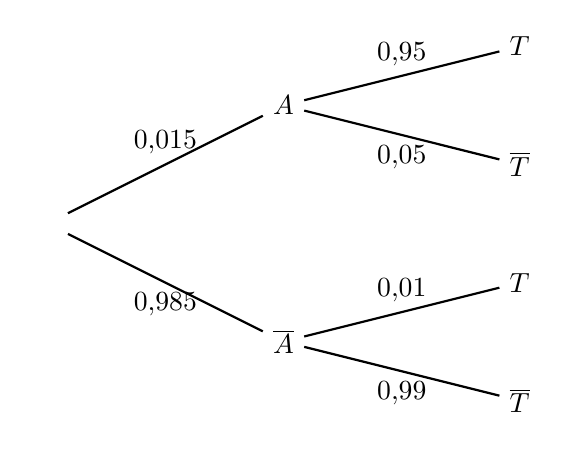
\begin{tikzpicture}[thick, scale=1.5] %{,}
\node (P_-1_0) at (-2,-1.5) {$\phantom{A}$};
\node (P_0_0) at (0,-0.5) {$A$};
\draw (P_-1_0) -- (P_0_0) node[midway, above] {$0{,}015$};
\node (P_1_0) at (2,-0) {$T$};
\draw (P_0_0) -- (P_1_0) node[midway, above] {$0{,}95$};
\node (P_1_1) at (2,-1) {$\overline{T}$};
\draw (P_0_0) -- (P_1_1) node[midway, below] {$0{,}05$};
\node (P_0_2) at (0,-2.5) {$\overline{A}$};
\draw (P_-1_0) -- (P_0_2) node[midway, below] {$0{,}985$};
\node (P_1_2) at (2,-2) {$T$};
\draw (P_0_2) -- (P_1_2) node[midway, above] {$0{,}01$};
\node (P_1_3) at (2,-3) {$\overline{T}$};
\draw (P_0_2) -- (P_1_3) node[midway, below] {$0{,}99$};
\end{tikzpicture}
\end{center}

Il faut trouver :
\[
P(T \cap \overline{A}) = P(\overline{A} \cap T) = P(\overline{A}) \times P_{\overline{A}}(T) = 0{,}985 \times 0{,}01 = 0{,}00985.
\]

\subsection*{2.}

On a de même :
\[
P(A \cap T) = P(A) \times P_A(T) = 0{,}015 \times 0{,}95 = 0{,}01425.
\]

D'après la loi des probabilités totales :
\[
P(T) = P(A \cap T) + P(T \cap \overline{A}) = 0{,}01425 + 0{,}00985 = 0{,}0241.
\]

\subsection*{3.}

On a :
\[
P_T(\overline{A}) = \dfrac{0{,}985 \times 0{,}05}{0{,}0635} = \dfrac{0{,}00985}{0{,}0241} \approx 0{,}4087.
\]

La probabilité sachant qu'une personne ayant été testée positive ne soit pas malade est d'environ \(0{,}409\) au millième près.

